\chapter{Der Tangentialraum}\lecture

Erinnerung (Diff 2): Sei $ M \subset \R^n $ eine Untermannigfaltigkeit, $p \in M$. Ein Tangentialvektor $v \in \R^n$ an $M$ in $p$ ist von der Form $ v = \gamma'(0) $, wobei $ \gamma: (-\epsilon,\epsilon) \to M $ mit $\gamma(0) = p$ eine in $M$ verlaufende $C^1$-Kurve ist. Der \emph{Tangentialraum} $T_pM$ (an $M$ in $p$) ist die Menge aller Tangentialvektoren. 
\begin{itemize}
	\item Ist $ U \subset \R^n $ offen, $p \in U$, $f: U \to \R^{n-m}$ $C^1$ mit $ M \cap U = \{x \in U \mid f(x) = 0\} $ und $rang(Df(p)) = n-m.$ Dann ist der Tangentialraum in $p$ an $M$ $ T_pM = \ker(Df(p)) \subset \R^n $ ($m$-dim. Unterraum).
	\item Ist $ \psi: V \to \R^n $ eine lokale Parametrisierung von $M$ bei $p$, so sind $ \del{j}\psi,\ d=1,\dotsc,m$, Basisvektoren $ V \subset \R^n $ für $ T_pM $.
\end{itemize}

\begin{exmp*}
	$ \Sbb^2 \subset \R^3,\ T_pM = p^\bot $, denn $ f: \R^n \to \R, f(x) = 1-\|x\|^2 $ für $ p \in \Sbb^2 $, sodass $p_i > 0$ oder $<0$ beschreibt $ \Sbb^2 \cap U_i \ni p, U_i = \{x \in \R^3 \mid x_i > 0 $ oder $ < 0\} $ als Nullstellengebilde und $ Df(p) = -2p. $
	\incfig{2}{14cm}
\end{exmp*}

Zur Verallgemeinerung auf Mannigfaltigkeiten\footnote{von nun an betrachten wir nur noch differenzierbare Mannigfaltigkeiten} überlegen wir zunächst, dass 2 Kurven zum selben Tangentialvektor führen, wenn sie in einer Umgebung von $p$ Übereinstimmen. Formalisiert und verallgemeinert führen wir daher ein:

\begin{defn}[Keime]\index{Keime}
	Auf $ \{f \mid f: U \to N,\ U $ offene Umgebung von $p \in M\} $ definiert 
	$$ f \sim g \iff \existss \text{offene Umgebung } V \ \text{von } p \text{, sodass } \bound{f}{V} = \bound{g}{V} $$
	eine Äquivalenzrelation. Eine Äquivalenzklasse bezüglich $\sim$ nennt man \emph{Keim} einer Abbildung $M \to N$ bei $p$. Ist $ f $ $C^1$/glatt bei $p$, so auch alle Elemente der von $f$ repräsentierten Klasse $\bar{f}$. Man spricht in dem Fall von $C^1$/glatten Keimen. Wir schreiben $ \Ecal^1(p) $ bzw. $\Ecal^\infty(p)$ für die Menge aller $C^1$ bzw. glatten Keime bei $p \in M$ mit Werten in $\R$ ("Funktionskeime") $ (M,p) \to \R $.
\end{defn}

\begin{rem}
	\begin{enumerate}[label={\roman*})]
		\item $\Ecal^1(p)$ und $\Ecal^\infty(p)$ bilden eine Algebra (denn die Bildung von Äquivalenzklassen ist mit der punktweisen Addition und Multiplikation verträglich).
		\item Ist $ \bar{f}: (M,p)\to N $ ein $C^1$/glatter Keim bei $p \in M$, so definiert er einen Homomorphismus von Algebren \big($\Ecal(f(p))$ Keime $(N,f(p)) \to \R$\big)
		\[ f^*: \Ecal^{1/\infty} (f(p)) \to \Ecal^{1/\infty} (p) \ \text{vermöge } f^* \big( \bar{h} \big) = \bar{h} \circ \bar{f} \quad \text{"pullback", "Zurückziehung"} \]
		Offensichtlich ist das unabhängig von der Wahl des Repräsentanten.
		\incfig{2_2}{14cm}
		Es gilt $\id^* = \id$ und $(f \circ g)^* = g^* \circ f^*$. Insbesondere induziert ein bezüglich Komposition invertierbarer Keim $\bar{f}$ ($ \bar{f} \circ \bar{f}^{-1} = \bar{f} \circ \overbar{f^{-1}} = \id $) einen Isomorphismus $f^*, f^{-1 *} \circ f^* = \id$.
		\item Spezialfall: Ist $\varphi$ eine um $p \in M$ zentrierte Karte, so definiert $\varphi$ einen invertierbaren Keim $ \overbar{\varphi}: (M,p) \to \R^n $ mit $\varphi(p)=0$ und somit einen Isomorphismus $ \varphi^*: \Ecal^{1/\infty}_n \to \Ecal^{1/\infty} (p) $, wobei $ \Ecal_n = \{$Funktionskeime bei $0 \}, $ das heißt man kann sich auf Keime aus $\Ecal_n$ beschränken.
	\end{enumerate}
\end{rem}

\section{3 Definitionen des Tangentialraums}

\begin{defn}[algebraische Definition]\index{Tangentialraum}\index{Derivation}
	Eine \emph{Derivation} von $\Ecal^\infty(p)$ ist eine lineare Abbildung $X: \Ecal^\infty(p) \to \R$, die der folgenden Leibniz-Regel genügt:
	\[ X(\bar{f} \cdot \bar{g}) = X(\bar{f}) \cdot g(p) + f(p) \cdot X(\bar{g}). \]
	Der \emph{Tangentialraum} $T_pM$ in $p$ ist der Vektorraum der Derivationen von $\Ecal^\infty(p)$.\\
	Ein glatter Keim $ \bar{f}: (M,p) \to N $ induziert einen Algebra-Homomorphismus $ f^*: \Ecal^\infty (f(p)) \to \Ecal^\infty (p) $ und somit eine (lineare) Abbildung, die \emph{Tangentialabbildung} (oder Differential) $ T_pf: T_pM \to T_{f(p)}N, X \mapsto X \circ f^*. $
\end{defn}

\begin{rem*}
	\begin{enumerate}[label={\roman*})]
		\item Es gilt 
		$$ T_p \big( \bar{g} \circ \bar{f} \big) = T_{f(p)} \bar{g} \circ T_p\bar{f}\quad \foralll \bar{f}: (M,p) \to N, \bar{g}: (N,f(p)) \to \tilde{N} \in C^\infty, $$
		denn für $\bar{h} \in \Ecal^\infty (g(f(p)))$ gilt
		\begin{align*}
			X \circ \Big( \big( \bar{g} \circ \bar{f} \big)^* \Big) \big( \bar{h} \big) &= X \big( \bar{h} \circ \big( \bar{g} \circ \bar{f} \big) \big)\\
			&= \big( X \circ f^* \big) \big( \bar{h} \circ \bar{g} \big)\\
			&= T_{f(p)}\bar{g} \big( X \circ f^* \big)(h)\\
			\text{und } \big( T_{f(p)} \bar{g} \circ T_p\bar{f} \big) &= T_{f(p)}\bar{g} \big( X \circ \bar{f}^* \big)\big( \bar{h} \big)
		\end{align*}
		\item Ist $\bar{\varphi}: (M,p) \to \R^n$ ein Keim einer bei $p$ zentrierten Karte, so ist $ \Ecal_n^\infty \overset{\cong}{\underset{\varphi^*}{\longrightarrow}} \Ecal^\infty(p) $ isomorph und $ T_pM \overset{\cong}{\underset{T_p \varphi}{\longrightarrow}} T_0\R^n $. 
	\end{enumerate}
\end{rem*}

$T_0\R^n$ hat eine besonders einfache Beschreibung:

\begin{lem}
	Die partiellen Ableitungen $ \del{j} $ in 0 bilden eine Basis von $ T_0\R^n. $
\end{lem}

\begin{rem*}
	$ \bound{\del{j}}{0} \overset{1:1}{\longleftrightarrow} e_j \in \R^n. $ Somit ist $ T_0\R^n \cong \R^n $ als Vektorraum.
\end{rem*}

\begin{thm}
	Seien $ (x_1,\dotsc,x_m),(y_1,\dotsc,y_n) $ lokale Koordinaten bei $p \in M, q \in N$, gegeben durch bei $p$ bzw. $q$ zentrierte Karten $ \varphi,\psi $ (das heißt $ x_i(\tilde{p}) = \varphi_i (\tilde{p}) $ mit $(\varphi,U)$ lokale Karte bei $p \in M, \tilde{p} \in U, \varphi(p) = 0$. Analog für $y_j$.)\\
	Dann sind $ \Big\{ \bound{\frac{\del{}}{\del{x_1}}}{0}, \dotsc, \bound{\frac{\del{}}{\del{x_m}}}{0} \Big\} $ bzw. $ \Big\{ \bound{\frac{\del{}}{\del{y_1}}}{0}, \dotsc, \bound{\frac{\del{}}{\del{y_n}}}{0} \Big\} $ Basen von $ T_0\R^m \cong T_pM $ bzw. $ T_0\R^n \cong T_qN $.\\
	Die Tangentialabbildung eines $C^\infty$-Keimes $\bar{f}: (M,p) \to N$ ist bezüglich dieser Basen durch die Jacobimatrix $ D( \vertarrowbox[1ex]{\psi \circ f \circ \varphi^{-1}}{Keim $ (\R^m,0) \to \R^n $} ) (0): \R^m \to \R^n $ gegeben.
	\[ \begin{tikzcd}
		T_pM \arrow{r}{Df} \arrow{d}{\varphi} & T_{f(p)}N \arrow{d}{\psi}\\
		T_0\R^m \arrow[r] & T_0\R^n
	\end{tikzcd} \]
\end{thm}

\begin{rem*}	
	Hierbei setzen wir $ \varphi^{-1} $ außerhalb von $ \varphi(U) $ glatt auf $\R^m$ fort.
\end{rem*}

\begin{exmp*}
	\begin{minipage}{\linewidth}
		\begin{wrapfigure}{R}{0.3\textwidth}
%			\centering
			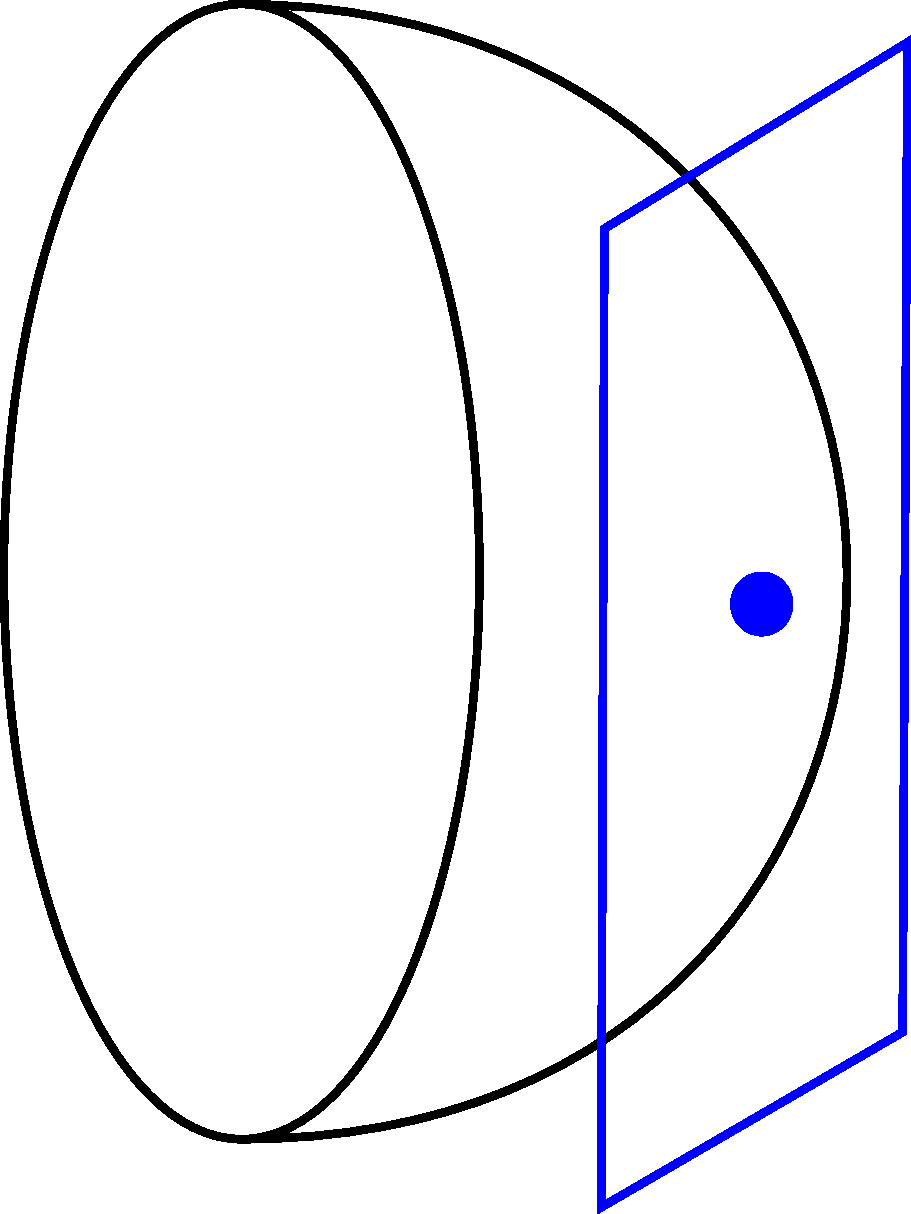
\includegraphics[width=0.1\textwidth]{2_5_1}
		\end{wrapfigure}
		$ M = \Sbb^1, p = (0,1,0)^T, \begin{aligned}[t]
			&\varphi: U_2^+ \cap \Sbb^2 \to \R^2, \\&\varphi(x) = (x_1,x_3)
		\end{aligned} $
	\end{minipage}
		
		Basis des Tangentialraums $ T_0\R^2 $ $ \bound{\del{1}}{0},\bound{\del{2}}{0} $\\
		$ f_{1,2}: \Sbb^2 \to \Sbb^2, \begin{aligned}[t]
			&f_1(x) = (x_1,-x_2,x_3),\\ &f_2(x) = (x_1,x_2,-x_3)
		\end{aligned} $\\
		$ \overbar{g_1} = \psi_1 \circ \overbar{f_1} \circ \varphi^{-1}: (\R^2,0) \to \R^2,\ \psi_1: U_2^- \cap \Sbb^2 \to \R^2, \psi_1 (x_1,x_2,x_3) = (x_1,x_3) $\\
		$ \overbar{g_2} = \psi_2 \circ \overbar{f_2} \circ \varphi^{-1}: (\R^2,0) \to \R^2,\ \psi_2 = \varphi $\\
		\begin{align*}
			Dg_j(0,0) &= D\psi_j (f_j(\overbrace{\varphi(0,0)}^{=p})) \circ Df_j(p) \circ D\varphi^{-1}(0,0)\\
			Dg_1(0,0) &= \begin{pmatrix}
					1&0&0\\0&0&0\\0&0&1
				\end{pmatrix} 
				\begin{pmatrix}
					1 & &\\&-1&\\&&1
				\end{pmatrix}
				\bound{\begin{pmatrix}
					1&0\\ \frac{-u_1}{\sqrt{1-\|u\|^2}} & \frac{-u_2}{\sqrt{1-\|u\|^2}} \\ 0&1
				\end{pmatrix}}{u=0} = 
				\begin{pmatrix}
					1&0\\0&0\\0&1
				\end{pmatrix}\\
			Dg_2(0,0) &= \begin{pmatrix}
					1&0&0\\0&0&0\\0&0&1
				\end{pmatrix} 
				\begin{pmatrix}
					1 & &\\&1&\\&&-1
				\end{pmatrix}
				\begin{pmatrix}
					1&0\\0&0\\0&1
				\end{pmatrix} = 
				\begin{pmatrix}
					1&0\\0&0\\0&-1
				\end{pmatrix}
		\end{align*}
\end{exmp*}

\subsection*{Verhalten unter Kartenwechseln}
	
	Seien $ \bar{\varphi},\bar{\psi}: (M,p) \to (\R^n,0) $ Kartenkeime. Dann ist der Kartenwechsel $ \Phi = \bar{\psi} \circ \bar{\varphi}^{-1}: (\R^m,0) \to \R^m $ ein glatter invertierbarer Keim und $\Phi$ ist eindeutig durch $ \psi,\varphi $ festgelegt. Solche $\Phi$ bilden eine Gruppe $\Gcal$ (bezüglich Komposition $\circ$). Durch die Zuordnung $ \Phi \mapsto D\Phi(0) $ erhält man einen Gruppenhomomorphismus $ \Gcal \to GL(m,\R) $.

\begin{defn}[physikalische Definition]\index{Tangentialraum}
	Ein \emph{Tangentialvektor} an $p \in M$ ($m$-dimensionale differenzierbare Mannigfaltigkeit) ist eine Zuordnung, die einem Kartenkeim $ \bar{\varphi}: (M,p) \to \R^m $ (einer bei $p$ zentrierten Karte) einen Vektor $v \in \R^m$ zuordnet, sodass $ \underbrace{(\overbar{\psi \circ \varphi^{-1}})}_{=\Phi} \circ \bar{\varphi} $ ($\psi$ weitere bei $p$ zentrierte Karte) der Vektor $D\Phi(0) \cdot v$ zugeordnet wird.
\end{defn}

\begin{lem}\label{2.7}
	$ (T_pM)_{phys} \cong T_pM $ (als Vektorräume)
\end{lem}

Schließlich die anschaulichste Definition:

\begin{defn}[geometrische Definition]\index{Tangentialraum}
	Sei $ \Gamma_p $ die Menge der glatten Keime $ \bar{\gamma}: (\R,0) \to M $ mit $\gamma(0) = p$. Wir definieren auf $\Gamma_p$ eine Äquivalenzrelation 
	\[ \overbar{\gamma_1} \sim \overbar{\gamma_2} \iff \frac{d}{d t}\big( \bar{f} \circ \overbar{\gamma_1} \big)(0) = \frac{d}{d t}\big( \bar{f} \circ \overbar{\gamma_2} \big)(0) \qquad \foralll \bar{f} \in \Ecal^\infty(p). \]
	Eine Äquivalenzklasse $[\gamma]$ ist ein Tangentialvektor $ \in (T_pM)_{geom} $.
	\image{2_8}{12cm}
\end{defn}

\begin{rem*}
	$ [\gamma] \mapsto X_\gamma,\ X_\gamma(\bar{f}) = \frac{d}{dt} \bar{f} \circ \bar{\gamma} (0) $ liefert eine bijektive Abbildung $ (T_pM)_{geom} \to T_pM $\\
	Injektivität: Nach Konstruktion sind für $ \tilde{\gamma} \notin [\gamma]: \frac{d}{dt}(\bar{f} \circ \bar{\gamma}) (0) \neq \frac{d}{dt}(\bar{f} \circ \bar{\tilde{\gamma}}) (0) $\\
	Surjektivität: Schreibt man $\gamma$ in lokalen Koordinaten $\gamma(t) = (ta_1,\dotsc,ta_m)$, so ist $X_\gamma = \sum_{i=1}^{m} a_i \bound{\del{i}}{0}.$
\end{rem*}

\begin{rem*}
	Tangentialabbildung:\\
	Sei $ \bar{f} : (M,p) \to N $ ein glatter Keim, dann ist $ \underbrace{[\gamma]}_{\in (T_pM)_{geom}} \mapsto \underbrace{[f \circ \gamma]}_{\in (T_{f(p)} N)_{geom}} $ die Tangentialabbildung $T_pf$, denn $\begin{aligned}[t]
		 X_{f \circ \gamma}(\bar{h}) &= \frac{d}{d t} (\bar{h} \circ \bar{f} \circ \bar{\gamma}) (0)\\
		 &= X_\gamma (\bar{h}\circ\bar{f})\\
		 &= T_pf(X_\gamma)(\bar{h}) 
	\end{aligned} \ \foralll \bar{h} \in \Ecal^\infty_{f(p)} $
	\image{2_8 rem}{14cm}
\end{rem*}

Wir werden im Folgenden die drei Definitionen des Tangentialraums je nach Praktikabilität verwenden und in der Notation nicht unterscheiden.

\begin{exmp*}
	Ist $V$ ein endlich-dimensionaler Vektorraum, so ist $V$ eine differenzierbare Mannigfaltigkeit. Die Wahl der Basis liefert einen Isomorphismus $ V \cong \R^n $ (Karte). Da lineare Abbildung $\R^n \to \R^n$ differenzierbar sind erhält man für jede Basis die selbe differenzierbare Struktur. Es gilt $ T_pV \cong V \ \foralll p. $ $ (v \in V, \gamma_v(t) = p + tv, [\gamma_v] \in T_pV) $
\end{exmp*}

